\documentclass{standalone}
\usepackage{tikz}
\usetikzlibrary{patterns, positioning}

\begin{document}
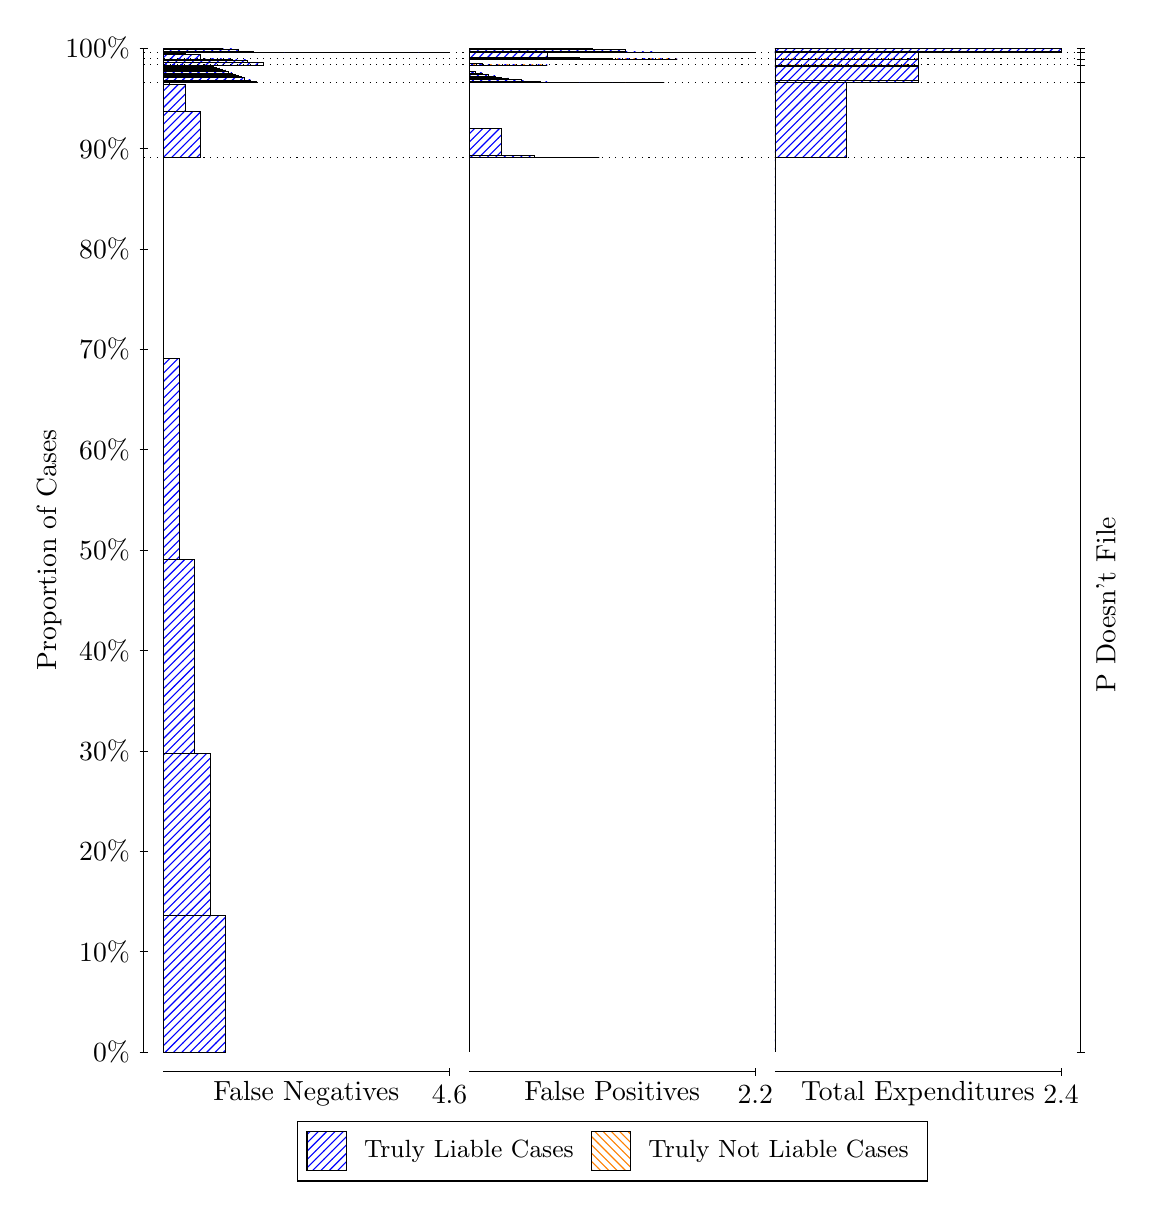
\begin{tikzpicture}
\draw[black, very thin] (1.5,1.75) -- (1.5,14.5);
\node[rotate=90, anchor=center] at (0.3, 8.125) {Proportion of Cases};
\draw[black, very thin] (1.45,1.75) -- (1.55,1.75);
\node[anchor=east] at (1.45, 1.75) {0\%};
\draw[black, very thin] (1.45,3.025) -- (1.55,3.025);
\node[anchor=east] at (1.45, 3.025) {10\%};
\draw[black, very thin] (1.45,4.3) -- (1.55,4.3);
\node[anchor=east] at (1.45, 4.3) {20\%};
\draw[black, very thin] (1.45,5.575) -- (1.55,5.575);
\node[anchor=east] at (1.45, 5.575) {30\%};
\draw[black, very thin] (1.45,6.85) -- (1.55,6.85);
\node[anchor=east] at (1.45, 6.85) {40\%};
\draw[black, very thin] (1.45,8.125) -- (1.55,8.125);
\node[anchor=east] at (1.45, 8.125) {50\%};
\draw[black, very thin] (1.45,9.4) -- (1.55,9.4);
\node[anchor=east] at (1.45, 9.4) {60\%};
\draw[black, very thin] (1.45,10.675) -- (1.55,10.675);
\node[anchor=east] at (1.45, 10.675) {70\%};
\draw[black, very thin] (1.45,11.95) -- (1.55,11.95);
\node[anchor=east] at (1.45, 11.95) {80\%};
\draw[black, very thin] (1.45,13.225) -- (1.55,13.225);
\node[anchor=east] at (1.45, 13.225) {90\%};
\draw[black, very thin] (1.45,14.5) -- (1.55,14.5);
\node[anchor=east] at (1.45, 14.5) {100\%};

\draw[black, very thin] (13.4,1.75) -- (13.4,14.5);
\draw[black, very thin] (13.35,1.75) -- (13.45,1.75);
\node[anchor=west] at (13.35, 1.75) {};
\draw[black, very thin] (13.35,13.108) -- (13.45,13.108);
\node[anchor=west] at (13.35, 13.108) {};
\draw[black, very thin] (13.35,14.064) -- (13.45,14.064);
\node[anchor=west] at (13.35, 14.064) {};
\draw[black, very thin] (13.35,14.287) -- (13.45,14.287);
\node[anchor=west] at (13.35, 14.287) {};
\draw[black, very thin] (13.35,14.363) -- (13.45,14.363);
\node[anchor=west] at (13.35, 14.363) {};
\draw[black, very thin] (13.35,14.44) -- (13.45,14.44);
\node[anchor=west] at (13.35, 14.44) {};
\draw[black, very thin] (13.35,14.5) -- (13.45,14.5);
\node[anchor=west] at (13.35, 14.5) {};

\draw[black, very thin, pattern color=blue, pattern=north east lines] (1.75,1.75) rectangle (2.5399,3.4867);
\draw[black, very thin, pattern color=blue, pattern=north east lines] (1.75,3.4867) rectangle (2.3424,5.5414);
\draw[black, very thin, pattern color=blue, pattern=north east lines] (1.75,5.5414) rectangle (2.1449,8.0083);
\draw[black, very thin, pattern color=blue, pattern=north east lines] (1.75,8.0083) rectangle (1.9475,10.558);
\draw[black, very thin, pattern color=orange, pattern=north west lines] (1.75,10.558) rectangle (1.75,10.558);
\draw[black, very thin, pattern color=blue, pattern=north east lines] (1.75,10.558) rectangle (1.75,13.108);
\draw[black, very thin, pattern color=blue, pattern=north east lines] (1.75,13.108) rectangle (2.2239,13.695);
\draw[black, very thin, pattern color=blue, pattern=north east lines] (1.75,13.695) rectangle (2.0264,14.04);
\draw[black, very thin, pattern color=blue, pattern=north east lines] (1.75,14.04) rectangle (1.829,14.064);
\draw[black, very thin, pattern color=orange, pattern=north west lines] (1.75,14.064) rectangle (1.75,14.064);
\draw[black, very thin, pattern color=blue, pattern=north east lines] (1.75,14.064) rectangle (1.75,14.064);
\draw[black, very thin, pattern color=blue, pattern=north east lines] (1.75,14.064) rectangle (2.9348,14.074);
\draw[black, very thin, pattern color=blue, pattern=north east lines] (1.75,14.074) rectangle (2.8558,14.095);
\draw[black, very thin, pattern color=blue, pattern=north east lines] (1.75,14.095) rectangle (2.7768,14.126);
\draw[black, very thin, pattern color=blue, pattern=north east lines] (1.75,14.126) rectangle (2.7373,14.138);
\draw[black, very thin, pattern color=blue, pattern=north east lines] (1.75,14.138) rectangle (2.6978,14.149);
\draw[black, very thin, pattern color=blue, pattern=north east lines] (1.75,14.149) rectangle (2.6583,14.166);
\draw[black, very thin, pattern color=blue, pattern=north east lines] (1.75,14.166) rectangle (2.6188,14.183);
\draw[black, very thin, pattern color=blue, pattern=north east lines] (1.75,14.183) rectangle (2.5793,14.204);
\draw[black, very thin, pattern color=blue, pattern=north east lines] (1.75,14.204) rectangle (2.5399,14.223);
\draw[black, very thin, pattern color=blue, pattern=north east lines] (1.75,14.223) rectangle (2.5004,14.23);
\draw[black, very thin, pattern color=blue, pattern=north east lines] (1.75,14.23) rectangle (2.4609,14.241);
\draw[black, very thin, pattern color=blue, pattern=north east lines] (1.75,14.241) rectangle (2.4609,14.247);
\draw[black, very thin, pattern color=blue, pattern=north east lines] (1.75,14.247) rectangle (2.4214,14.255);
\draw[black, very thin, pattern color=blue, pattern=north east lines] (1.75,14.255) rectangle (2.3819,14.263);
\draw[black, very thin, pattern color=blue, pattern=north east lines] (1.75,14.263) rectangle (2.3819,14.268);
\draw[black, very thin, pattern color=blue, pattern=north east lines] (1.75,14.268) rectangle (2.3424,14.272);
\draw[black, very thin, pattern color=blue, pattern=north east lines] (1.75,14.272) rectangle (2.3029,14.278);
\draw[black, very thin, pattern color=blue, pattern=north east lines] (1.75,14.278) rectangle (2.2634,14.281);
\draw[black, very thin, pattern color=blue, pattern=north east lines] (1.75,14.281) rectangle (2.2634,14.281);
\draw[black, very thin, pattern color=blue, pattern=north east lines] (1.75,14.281) rectangle (2.2239,14.283);
\draw[black, very thin, pattern color=blue, pattern=north east lines] (1.75,14.283) rectangle (2.1844,14.283);
\draw[black, very thin, pattern color=blue, pattern=north east lines] (1.75,14.283) rectangle (2.1844,14.285);
\draw[black, very thin, pattern color=blue, pattern=north east lines] (1.75,14.285) rectangle (2.1449,14.285);
\draw[black, very thin, pattern color=blue, pattern=north east lines] (1.75,14.285) rectangle (2.1054,14.285);
\draw[black, very thin, pattern color=blue, pattern=north east lines] (1.75,14.285) rectangle (2.1054,14.287);
\draw[black, very thin, pattern color=blue, pattern=north east lines] (1.75,14.287) rectangle (2.0659,14.287);
\draw[black, very thin, pattern color=blue, pattern=north east lines] (1.75,14.287) rectangle (2.0659,14.287);
\draw[black, very thin, pattern color=blue, pattern=north east lines] (1.75,14.287) rectangle (2.0264,14.287);
\draw[black, very thin, pattern color=blue, pattern=north east lines] (1.75,14.287) rectangle (1.987,14.287);
\draw[black, very thin, pattern color=blue, pattern=north east lines] (1.75,14.287) rectangle (1.987,14.287);
\draw[black, very thin, pattern color=blue, pattern=north east lines] (1.75,14.287) rectangle (1.9475,14.287);
\draw[black, very thin, pattern color=blue, pattern=north east lines] (1.75,14.287) rectangle (1.908,14.287);
\draw[black, very thin, pattern color=blue, pattern=north east lines] (1.75,14.287) rectangle (1.908,14.287);
\draw[black, very thin, pattern color=blue, pattern=north east lines] (1.75,14.287) rectangle (1.8685,14.287);
\draw[black, very thin, pattern color=blue, pattern=north east lines] (1.75,14.287) rectangle (1.829,14.287);
\draw[black, very thin, pattern color=blue, pattern=north east lines] (1.75,14.287) rectangle (1.7895,14.287);
\draw[black, very thin, pattern color=orange, pattern=north west lines] (1.75,14.287) rectangle (1.75,14.287);
\draw[black, very thin, pattern color=blue, pattern=north east lines] (1.75,14.287) rectangle (1.75,14.287);
\draw[black, very thin, pattern color=blue, pattern=north east lines] (1.75,14.287) rectangle (3.0138,14.32);
\draw[black, very thin, pattern color=blue, pattern=north east lines] (1.75,14.32) rectangle (2.8163,14.348);
\draw[black, very thin, pattern color=blue, pattern=north east lines] (1.75,14.348) rectangle (2.6188,14.363);
\draw[black, very thin, pattern color=blue, pattern=north east lines] (1.75,14.363) rectangle (2.4214,14.363);
\draw[black, very thin, pattern color=blue, pattern=north east lines] (1.75,14.363) rectangle (2.2239,14.363);
\draw[black, very thin, pattern color=orange, pattern=north west lines] (1.75,14.363) rectangle (1.75,14.363);
\draw[black, very thin, pattern color=blue, pattern=north east lines] (1.75,14.363) rectangle (2.2239,14.417);
\draw[black, very thin, pattern color=blue, pattern=north east lines] (1.75,14.417) rectangle (2.0264,14.438);
\draw[black, very thin, pattern color=blue, pattern=north east lines] (1.75,14.438) rectangle (1.829,14.44);
\draw[black, very thin, pattern color=orange, pattern=north west lines] (1.75,14.44) rectangle (1.75,14.44);
\draw[black, very thin, pattern color=blue, pattern=north east lines] (1.75,14.44) rectangle (1.75,14.44);
\draw[black, very thin, pattern color=blue, pattern=north east lines] (1.75,14.44) rectangle (5.3833,14.44);
\draw[black, very thin, pattern color=blue, pattern=north east lines] (1.75,14.44) rectangle (5.1859,14.44);
\draw[black, very thin, pattern color=blue, pattern=north east lines] (1.75,14.44) rectangle (4.9884,14.44);
\draw[black, very thin, pattern color=blue, pattern=north east lines] (1.75,14.44) rectangle (4.7909,14.443);
\draw[black, very thin, pattern color=blue, pattern=north east lines] (1.75,14.443) rectangle (4.5935,14.443);
\draw[black, very thin, pattern color=blue, pattern=north east lines] (1.75,14.443) rectangle (4.396,14.443);
\draw[black, very thin, pattern color=blue, pattern=north east lines] (1.75,14.443) rectangle (4.1986,14.443);
\draw[black, very thin, pattern color=blue, pattern=north east lines] (1.75,14.443) rectangle (3.2902,14.443);
\draw[black, very thin, pattern color=blue, pattern=north east lines] (1.75,14.443) rectangle (3.0928,14.444);
\draw[black, very thin, pattern color=blue, pattern=north east lines] (1.75,14.444) rectangle (2.8953,14.457);
\draw[black, very thin, pattern color=blue, pattern=north east lines] (1.75,14.457) rectangle (2.6978,14.49);
\draw[black, very thin, pattern color=blue, pattern=north east lines] (1.75,14.49) rectangle (2.5004,14.5);
\draw[black, very thin, pattern color=blue, pattern=north east lines] (1.75,14.5) rectangle (2.3029,14.5);
\draw[black, very thin, pattern color=blue, pattern=north east lines] (1.75,14.5) rectangle (2.1054,14.5);
\draw[black, very thin, pattern color=blue, pattern=north east lines] (1.75,14.5) rectangle (1.908,14.5);
\draw[black, very thin, pattern color=orange, pattern=north west lines] (1.75,14.5) rectangle (1.75,14.5);
\draw[black, very thin, pattern color=orange, pattern=north west lines] (5.6333,1.75) rectangle (5.6333,1.75);
\draw[black, very thin, pattern color=blue, pattern=north east lines] (5.6333,1.75) rectangle (5.6333,13.108);
\draw[black, very thin, pattern color=orange, pattern=north west lines] (5.6333,13.108) rectangle (7.2848,13.108);
\draw[black, very thin, pattern color=blue, pattern=north east lines] (5.6333,13.108) rectangle (7.2848,13.108);
\draw[black, very thin, pattern color=blue, pattern=north east lines] (5.6333,13.108) rectangle (6.872,13.108);
\draw[black, very thin, pattern color=blue, pattern=north east lines] (5.6333,13.108) rectangle (6.4591,13.132);
\draw[black, very thin, pattern color=blue, pattern=north east lines] (5.6333,13.132) rectangle (6.0462,13.477);
\draw[black, very thin, pattern color=blue, pattern=north east lines] (5.6333,13.477) rectangle (5.6333,14.064);
\draw[black, very thin, pattern color=orange, pattern=north west lines] (5.6333,14.064) rectangle (8.1106,14.064);
\draw[black, very thin, pattern color=blue, pattern=north east lines] (5.6333,14.064) rectangle (8.1106,14.064);
\draw[black, very thin, pattern color=orange, pattern=north west lines] (5.6333,14.064) rectangle (7.9455,14.064);
\draw[black, very thin, pattern color=blue, pattern=north east lines] (5.6333,14.064) rectangle (7.9455,14.064);
\draw[black, very thin, pattern color=orange, pattern=north west lines] (5.6333,14.064) rectangle (7.7803,14.064);
\draw[black, very thin, pattern color=blue, pattern=north east lines] (5.6333,14.064) rectangle (7.7803,14.064);
\draw[black, very thin, pattern color=blue, pattern=north east lines] (5.6333,14.064) rectangle (7.6977,14.064);
\draw[black, very thin, pattern color=orange, pattern=north west lines] (5.6333,14.064) rectangle (7.6152,14.064);
\draw[black, very thin, pattern color=blue, pattern=north east lines] (5.6333,14.064) rectangle (7.6152,14.064);
\draw[black, very thin, pattern color=blue, pattern=north east lines] (5.6333,14.064) rectangle (7.5326,14.064);
\draw[black, very thin, pattern color=orange, pattern=north west lines] (5.6333,14.064) rectangle (7.45,14.064);
\draw[black, very thin, pattern color=blue, pattern=north east lines] (5.6333,14.064) rectangle (7.45,14.064);
\draw[black, very thin, pattern color=blue, pattern=north east lines] (5.6333,14.064) rectangle (7.3674,14.064);
\draw[black, very thin, pattern color=orange, pattern=north west lines] (5.6333,14.064) rectangle (7.2848,14.064);
\draw[black, very thin, pattern color=blue, pattern=north east lines] (5.6333,14.064) rectangle (7.2848,14.064);
\draw[black, very thin, pattern color=blue, pattern=north east lines] (5.6333,14.064) rectangle (7.2023,14.064);
\draw[black, very thin, pattern color=orange, pattern=north west lines] (5.6333,14.064) rectangle (7.1197,14.064);
\draw[black, very thin, pattern color=blue, pattern=north east lines] (5.6333,14.064) rectangle (7.1197,14.064);
\draw[black, very thin, pattern color=blue, pattern=north east lines] (5.6333,14.064) rectangle (7.0371,14.064);
\draw[black, very thin, pattern color=orange, pattern=north west lines] (5.6333,14.064) rectangle (6.9545,14.064);
\draw[black, very thin, pattern color=blue, pattern=north east lines] (5.6333,14.064) rectangle (6.9545,14.064);
\draw[black, very thin, pattern color=blue, pattern=north east lines] (5.6333,14.064) rectangle (6.9545,14.065);
\draw[black, very thin, pattern color=blue, pattern=north east lines] (5.6333,14.065) rectangle (6.872,14.066);
\draw[black, very thin, pattern color=orange, pattern=north west lines] (5.6333,14.066) rectangle (6.7894,14.066);
\draw[black, very thin, pattern color=blue, pattern=north east lines] (5.6333,14.066) rectangle (6.7894,14.066);
\draw[black, very thin, pattern color=blue, pattern=north east lines] (5.6333,14.066) rectangle (6.7068,14.068);
\draw[black, very thin, pattern color=blue, pattern=north east lines] (5.6333,14.068) rectangle (6.6242,14.07);
\draw[black, very thin, pattern color=blue, pattern=north east lines] (5.6333,14.07) rectangle (6.5417,14.07);
\draw[black, very thin, pattern color=blue, pattern=north east lines] (5.6333,14.07) rectangle (6.5417,14.074);
\draw[black, very thin, pattern color=blue, pattern=north east lines] (5.6333,14.074) rectangle (6.4591,14.08);
\draw[black, very thin, pattern color=blue, pattern=north east lines] (5.6333,14.08) rectangle (6.3765,14.084);
\draw[black, very thin, pattern color=blue, pattern=north east lines] (5.6333,14.084) rectangle (6.2939,14.097);
\draw[black, very thin, pattern color=blue, pattern=north east lines] (5.6333,14.097) rectangle (6.2114,14.105);
\draw[black, very thin, pattern color=blue, pattern=north east lines] (5.6333,14.105) rectangle (6.1288,14.111);
\draw[black, very thin, pattern color=blue, pattern=north east lines] (5.6333,14.111) rectangle (6.1288,14.121);
\draw[black, very thin, pattern color=blue, pattern=north east lines] (5.6333,14.121) rectangle (6.0462,14.128);
\draw[black, very thin, pattern color=blue, pattern=north east lines] (5.6333,14.128) rectangle (5.9636,14.147);
\draw[black, very thin, pattern color=blue, pattern=north east lines] (5.6333,14.147) rectangle (5.8811,14.169);
\draw[black, very thin, pattern color=blue, pattern=north east lines] (5.6333,14.169) rectangle (5.7985,14.185);
\draw[black, very thin, pattern color=blue, pattern=north east lines] (5.6333,14.185) rectangle (5.7159,14.203);
\draw[black, very thin, pattern color=blue, pattern=north east lines] (5.6333,14.203) rectangle (5.6333,14.287);
\draw[black, very thin, pattern color=orange, pattern=north west lines] (5.6333,14.287) rectangle (6.6242,14.287);
\draw[black, very thin, pattern color=blue, pattern=north east lines] (5.6333,14.287) rectangle (6.6242,14.287);
\draw[black, very thin, pattern color=blue, pattern=north east lines] (5.6333,14.287) rectangle (6.2114,14.287);
\draw[black, very thin, pattern color=blue, pattern=north east lines] (5.6333,14.287) rectangle (5.7985,14.302);
\draw[black, very thin, pattern color=blue, pattern=north east lines] (5.6333,14.302) rectangle (5.6333,14.363);
\draw[black, very thin, pattern color=orange, pattern=north west lines] (5.6333,14.363) rectangle (8.2758,14.363);
\draw[black, very thin, pattern color=blue, pattern=north east lines] (5.6333,14.363) rectangle (8.2758,14.363);
\draw[black, very thin, pattern color=blue, pattern=north east lines] (5.6333,14.363) rectangle (7.8629,14.363);
\draw[black, very thin, pattern color=blue, pattern=north east lines] (5.6333,14.363) rectangle (7.45,14.365);
\draw[black, very thin, pattern color=blue, pattern=north east lines] (5.6333,14.365) rectangle (7.0371,14.385);
\draw[black, very thin, pattern color=blue, pattern=north east lines] (5.6333,14.385) rectangle (6.6242,14.44);
\draw[black, very thin, pattern color=orange, pattern=north west lines] (5.6333,14.44) rectangle (9.2667,14.44);
\draw[black, very thin, pattern color=blue, pattern=north east lines] (5.6333,14.44) rectangle (9.2667,14.44);
\draw[black, very thin, pattern color=blue, pattern=north east lines] (5.6333,14.44) rectangle (8.8538,14.44);
\draw[black, very thin, pattern color=orange, pattern=north west lines] (5.6333,14.44) rectangle (8.8538,14.44);
\draw[black, very thin, pattern color=blue, pattern=north east lines] (5.6333,14.44) rectangle (8.8538,14.44);
\draw[black, very thin, pattern color=blue, pattern=north east lines] (5.6333,14.44) rectangle (8.4409,14.44);
\draw[black, very thin, pattern color=orange, pattern=north west lines] (5.6333,14.44) rectangle (8.4409,14.44);
\draw[black, very thin, pattern color=blue, pattern=north east lines] (5.6333,14.44) rectangle (8.4409,14.44);
\draw[black, very thin, pattern color=blue, pattern=north east lines] (5.6333,14.44) rectangle (8.028,14.446);
\draw[black, very thin, pattern color=orange, pattern=north west lines] (5.6333,14.446) rectangle (8.028,14.446);
\draw[black, very thin, pattern color=blue, pattern=north east lines] (5.6333,14.446) rectangle (8.028,14.45);
\draw[black, very thin, pattern color=blue, pattern=north east lines] (5.6333,14.45) rectangle (7.6152,14.462);
\draw[black, very thin, pattern color=blue, pattern=north east lines] (5.6333,14.462) rectangle (7.6152,14.482);
\draw[black, very thin, pattern color=blue, pattern=north east lines] (5.6333,14.482) rectangle (7.2023,14.495);
\draw[black, very thin, pattern color=blue, pattern=north east lines] (5.6333,14.495) rectangle (6.7894,14.496);
\draw[black, very thin, pattern color=blue, pattern=north east lines] (5.6333,14.496) rectangle (6.3765,14.496);
\draw[black, very thin, pattern color=orange, pattern=north west lines] (5.6333,14.496) rectangle (5.6333,14.496);
\draw[black, very thin, pattern color=blue, pattern=north east lines] (5.6333,14.496) rectangle (5.6333,14.5);
\draw[black, very thin, pattern color=orange, pattern=north west lines] (9.5167,1.75) rectangle (9.5167,1.75);
\draw[black, very thin, pattern color=blue, pattern=north east lines] (9.5167,1.75) rectangle (9.5167,13.108);
\draw[black, very thin, pattern color=orange, pattern=north west lines] (9.5167,13.108) rectangle (10.425,13.108);
\draw[black, very thin, pattern color=blue, pattern=north east lines] (9.5167,13.108) rectangle (10.425,14.064);
\draw[black, very thin, pattern color=orange, pattern=north west lines] (9.5167,14.064) rectangle (11.333,14.064);
\draw[black, very thin, pattern color=blue, pattern=north east lines] (9.5167,14.064) rectangle (11.333,14.091);
\draw[black, very thin, pattern color=orange, pattern=north west lines] (9.5167,14.091) rectangle (11.333,14.091);
\draw[black, very thin, pattern color=blue, pattern=north east lines] (9.5167,14.091) rectangle (11.333,14.267);
\draw[black, very thin, pattern color=orange, pattern=north west lines] (9.5167,14.267) rectangle (11.333,14.267);
\draw[black, very thin, pattern color=blue, pattern=north east lines] (9.5167,14.267) rectangle (11.333,14.287);
\draw[black, very thin, pattern color=orange, pattern=north west lines] (9.5167,14.287) rectangle (11.333,14.287);
\draw[black, very thin, pattern color=blue, pattern=north east lines] (9.5167,14.287) rectangle (11.333,14.363);
\draw[black, very thin, pattern color=orange, pattern=north west lines] (9.5167,14.363) rectangle (11.333,14.363);
\draw[black, very thin, pattern color=blue, pattern=north east lines] (9.5167,14.363) rectangle (11.333,14.44);
\draw[black, very thin, pattern color=orange, pattern=north west lines] (9.5167,14.44) rectangle (13.15,14.44);
\draw[black, very thin, pattern color=blue, pattern=north east lines] (9.5167,14.44) rectangle (13.15,14.459);
\draw[black, very thin, pattern color=orange, pattern=north west lines] (9.5167,14.459) rectangle (13.15,14.459);
\draw[black, very thin, pattern color=blue, pattern=north east lines] (9.5167,14.459) rectangle (13.15,14.496);
\draw[black, very thin, pattern color=orange, pattern=north west lines] (9.5167,14.496) rectangle (13.15,14.496);
\draw[black, very thin, pattern color=blue, pattern=north east lines] (9.5167,14.496) rectangle (13.15,14.5);
\draw[black, dotted] (1.5,13.108) -- (13.4,13.108);
\draw[black, dotted] (1.5,14.064) -- (13.4,14.064);
\draw[black, dotted] (1.5,14.287) -- (13.4,14.287);
\draw[black, dotted] (1.5,14.363) -- (13.4,14.363);
\draw[black, dotted] (1.5,14.44) -- (13.4,14.44);
\draw[black, very thin] (1.75,1.5) -- (5.3833,1.5);
\node[anchor=north] at (3.5667, 1.5) {False Negatives};
\draw[black, very thin] (5.3833,1.45) -- (5.3833,1.55);
\node[anchor=north] at (5.3833, 1.45) {4.6};

\draw[black, very thin] (5.6333,1.5) -- (9.2667,1.5);
\node[anchor=north] at (7.45, 1.5) {False Positives};
\draw[black, very thin] (9.2667,1.45) -- (9.2667,1.55);
\node[anchor=north] at (9.2667, 1.45) {2.2};

\draw[black, very thin] (9.5167,1.5) -- (13.15,1.5);
\node[anchor=north] at (11.333, 1.5) {Total Expenditures};
\draw[black, very thin] (13.15,1.45) -- (13.15,1.55);
\node[anchor=north] at (13.15, 1.45) {2.4};

\node[black, centered, rotate=90] at (13.72, 7.4288) {P Doesn't File};






\draw (7.449999999999999,1.5) node[draw=none] (baseCoordinate) {};
\begin{scope}[align=center]
        \matrix[scale=0.5, draw=black, below=0.5cm of baseCoordinate, nodes={draw}, column sep=0.1cm]{
            \node[rectangle, draw, minimum width=0.5cm, minimum height=0.5cm, pattern=north east lines, pattern color=blue] {}; &
            \node[draw=none, font=\small] (B) {Truly Liable Cases}; &
            \node[rectangle, draw, minimum width=0.5cm, minimum height=0.5cm, pattern=north west lines, pattern color=orange] {}; &
            \node[draw=none, font=\small] (B) {Truly Not Liable Cases}; \\
            };
\end{scope}

\end{tikzpicture}
\end{document}